\subsection{Nozzle [Gabriel Diez]}

An aerospike nozzle design was chosen to expand the gases exiting the combustor and add additional thrust. Imbaratto \cite{imbaratto} specifies a method to design the contour of an ideally expanded aerospike nozzle utilizing the Prandtl-Meyer function. The method starts by calculating the nozzle pressure ratio. Normally nozzles are designed for a combustor with a constant chamber pressure, however, in an RDE engine the pressure varies with time and location as a result of the travelling detonation wave. Therefore, the average pressure over the whole nozzle entrance area was calculated to be 365.8 kPa. Based on this pressure and the combustor exit Mach number and temperature of 2.14 and 2417 K, respectively, the Prandtl-Meyer function was solved to find the maximum turning angle of the flow at several points. A MATLAB program was then made to plot these points, developing the nozzle contour along the axial length from the combustor.

\begin{wrapfigure}{r}{0.6\textwidth}
\begin{center}
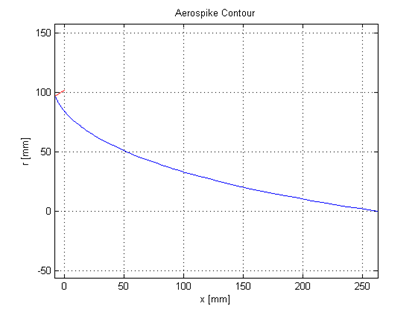
\includegraphics[width=0.6\textwidth]{aerospikeContour}
\caption{Aerospike Contour}
\label{fig:aerospikeContour}
\end{center}
\end{wrapfigure}
 
The result of this is shown in Figure \ref{fig:aerospikeContour} and it is apparent that the ideal contour leads to a long and sharp tip. While this thin tip does lead to perfect expansion to ambient pressure, it is impractical for several reasons. Manufacturing a shrinking spike with a precise geometry such as this would be difficult and the pointed end could be easily damaged. The main problem with the purely ideal aerospike nozzle, however, is heat transfer. Developing a system to effectively remove the heat being deposited in a 2 mm diameter pointed spike by supersonic gas at the high temperatures exhibited by a scramjet would be far too strenuous to justify the negligible improvement in expansion it would provide. The static pressure as a function of distance long the nozzle was then calculated and plotted in Figure \ref{fig:aerospikePressure}. A point 127 mm in length and 25 mm in radius was chosen to truncate the nozzle as it would only leave the exiting flow with a static pressure of about 3 KPa above ambient which was deemed acceptable. The final nozzle design is displayed in Figure \ref{fig:nozzleIsoView}.

\begin{figure}[H]
\begin{center}
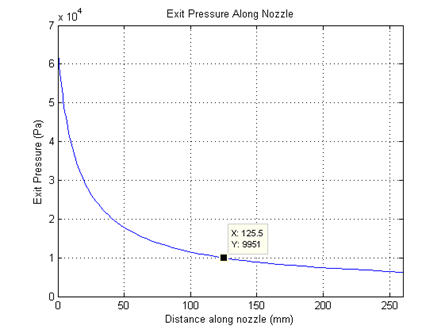
\includegraphics[width=0.6\textwidth]{aerospikePressure}
\caption{Pressure Along the Aerospike}
\label{fig:aerospikePressure}
\end{center}
\end{figure}


